\chapter*{Dodatak: Prikaz aktivnosti grupe}
	\addcontentsline{toc}{chapter}{Dodatak: Prikaz aktivnosti grupe}
	
		\section*{Dnevnik sastajanja}
		
		\textbf{\textit{Kontinuirano osvježavanje}}\\
		
		\textit{U ovom dijelu potrebno je redovito osvježavati dnevnik sastajanja prema predlošku.}
		
		\begin{packed_enum}
			\item  sastanak
			
			\item[] \begin{packed_item}
				\item Datum: 16. listopada 2023.
				\item Prisustvovali: D. Agejev, M. Haralović, I. Skukan, L. Galiot, M. Lovrinović, N. Vidović, T. Tomić
				\item Teme sastanka:
				\begin{packed_item}
					\item  Upoznavanje
					\item  Kompetencije i želje
					\item  Prijedlozi tehnologija
				\end{packed_item}
			\end{packed_item}
			
			\item  sastanak
			\item[] \begin{packed_item}
				\item Datum: 21. listopada 2023.
				\item Prisustvovali:  D. Agejev, M. Haralović, I. Skukan, L. Galiot, M. Lovrinović, N. Vidović, T. Tomić
				\item Teme sastanka:
				\begin{packed_item}
					\item  Pregled zadatka
					\item  Utvrđene uloge u razvoju
					\item  Odabir tehnologija
					\item  Raspodjela zadataka za dokumentaciju
					\item  Raspravljanje o nejasnoćama i implementaciji zadatka
				\end{packed_item}
			\end{packed_item}
			
			\item  sastanak
			\item[] \begin{packed_item}
				\item Datum: 23. listopada 2023.
				\item Prisustvovali:  D. Agejev, prof. Jović
				\item Teme sastanka:
				\begin{packed_item}
					\item  Razjašnjavanje nejasnoća oko zadatka
					\begin{packed_item}
						\item  Generička funkcionalnost
						\item  Apstrahiranje vrsta knjiga
						\item  Elementi opisa zadatka
						\item  Opis arhitekture sustava
					\end{packed_item}
				\end{packed_item}
			\end{packed_item}
			
			\item  sastanak
			\item[] \begin{packed_item}
				\item Datum: 28. listopada 2023.
				\item Prisustvovali:  D. Agejev, M. Haralović, I. Skukan, L. Galiot, M. Lovrinović, N. Vidović, T. Tomić
				\item Teme sastanka:
				\begin{packed_item}
					\item  Upute za GitHub
				\end{packed_item}
			\end{packed_item}
			
			\item  sastanak
			\item[] \begin{packed_item}
				\item Datum: 30. listopada 2023.
				\item Prisustvovali:  D. Agejev, prof. Jović
				\item Teme sastanka:
				\begin{packed_item}
					\item  Razjašnjavanje nejasnoća oko zadatka
					\begin{packed_item}
						\item  Odobravanje registracija
						\item  Zahtjevi za prijevod
						\item  GitHub feature grane
					\end{packed_item}
				\end{packed_item}
			\end{packed_item}
			
			\item  sastanak
			\item[] \begin{packed_item}
				\item Datum: 31. listopada 2023.
				\item Prisustvovali:  D. Agejev, M. Haralović, I. Skukan
				\item Teme sastanka:
				\begin{packed_item}
					\item  Pregled prototipa korisničkog sučelja
				\end{packed_item}
			\end{packed_item}
			
			\item  sastanak
			\item[] \begin{packed_item}
				\item Datum: 18. siječnja 2024.
				\item Prisustvovali:  D. Agejev, M. Haralović, I. Skukan, M. Lovrinović
				\item Teme sastanka:
				\begin{packed_item}
					\item  Pregled korisničkog sučelja
					\item  Ispitivanje funkcionalnosti
					\item  Utvrđivanje popravaka i mogućih nadogradnji
				\end{packed_item}
			\end{packed_item}
			
			%
			
		\end{packed_enum}
		
		\eject
		\section*{Tablica aktivnosti}

			\begin{longtblr}[
					label=none,
				]{
					vlines,hlines,
					width = \textwidth,
					colspec={X[7, l]X[1, c]X[1, c]X[1, c]X[1, c]X[1, c]X[1, c]X[1, c]}, 
					vline{1} = {1}{text=\clap{}},
					hline{1} = {1}{text=\clap{}},
					rowhead = 1,
				} 
			
				\SetCell[c=1]{c}{} & \SetCell[c=1]{c}{\rotatebox{90}{\textbf{Dominik Agejev }}} & \SetCell[c=1]{c}{\rotatebox{90}{\textbf{Marko Haralović }}} &	\SetCell[c=1]{c}{\rotatebox{90}{\textbf{Ivan Skukan }}} & \SetCell[c=1]{c}{\rotatebox{90}{\textbf{Lovro Galiot }}} &	\SetCell[c=1]{c}{\rotatebox{90}{\textbf{Marin Lovrinović }}} & \SetCell[c=1]{c}{\rotatebox{90}{\textbf{Niko Vidović }}} &	\SetCell[c=1]{c}{\rotatebox{90}{\textbf{Tvrtko Tomić }}} \\  
				Upravljanje projektom 		& 19 &  &  &  &  &  & \\ 
				Opis projektnog zadatka 	& 3 & 10 &  &  &  &  & \\ 
				
				Funkcionalni zahtjevi       &  &  & 8 & 4 &  &  &  \\ 
				Opis pojedinih obrazaca 	&  &  & 4 & 2 &  &  &  \\ 
				Dijagram obrazaca 			&  &  & 5 & 2 &  &  &  \\ 
				Sekvencijski dijagrami 		&  &  &  &  & 4 & 8 & \\ 
				Opis ostalih zahtjeva 		& 1 &  &  &  &  &  &  \\ 

				Arhitektura i dizajn sustava	 & 2 &  &  &  &  3  &  \\ 
				Baza podataka				&  &  &  &  & 1 & & 13  \\ 
				Dijagram razreda 			&  &  &  &  &  & 9 &   \\ 
				Dijagram stanja				&  &  &  &  &  &  &  \\ 
				Dijagram aktivnosti 		&  &  &  &  &  & 4 &  \\ 
				Dijagram komponenti			&  &  &  &  &  & 2 &  \\ 
				Korištene tehnologije i alati 		& 2 & 1 &  &  &  3  &  \\ 
				Ispitivanje programskog rješenja 	& 2 &  &  &  &  1  &  \\ 
				Dijagram razmještaja			&  &  &  &  &  &  & 3 \\ 
				Upute za puštanje u pogon 		&  & 3 &  &  &  &  &  \\  
				Dnevnik sastajanja 			& 2 &  &  &  &  &  &  \\ 
				Zaključak i budući rad 		&  &  &  &  &  &  &  \\  
				Popis literature 			& 1 &  &  &  &  &  &  \\ 
				 
				Izrada početne stranice		& 1 &  & 5 & 7 &  1  &  \\ 
				Stranice za objave			&  &  & 3 & 5 &  &  &  \\  
				Stranica za novu objavu		&  &  & 2 & 3 &  &  &  \\  
				Stranice za login i registraciju 	& 2 &  & 5 & 2 &  &  &  \\  
				Stranica za pregled računa	&  &  & 2 & 2 &  &  &  \\  
				Izrada skripti za funkcionalnost stranice 	&  &  & 4 & 6 &  &  &  \\  
				Omogućavanje responzivnosti stranice 	& 1 &  & 3 & 5 &  & 1 &  \\  
				Izrada baze podataka 		 			&  &  &  &  & 1 & & 6\\  
				Spajanje s bazom podataka 							&  & 2 &  &  & 1 &  \\ 
				Back end 							&  &  &  &  & 39 &  \\
			\end{longtblr}
					
					
		\eject
		\section*{Dijagrami pregleda promjena}
		
		\begin{figure}[hbt!]
			\centering
			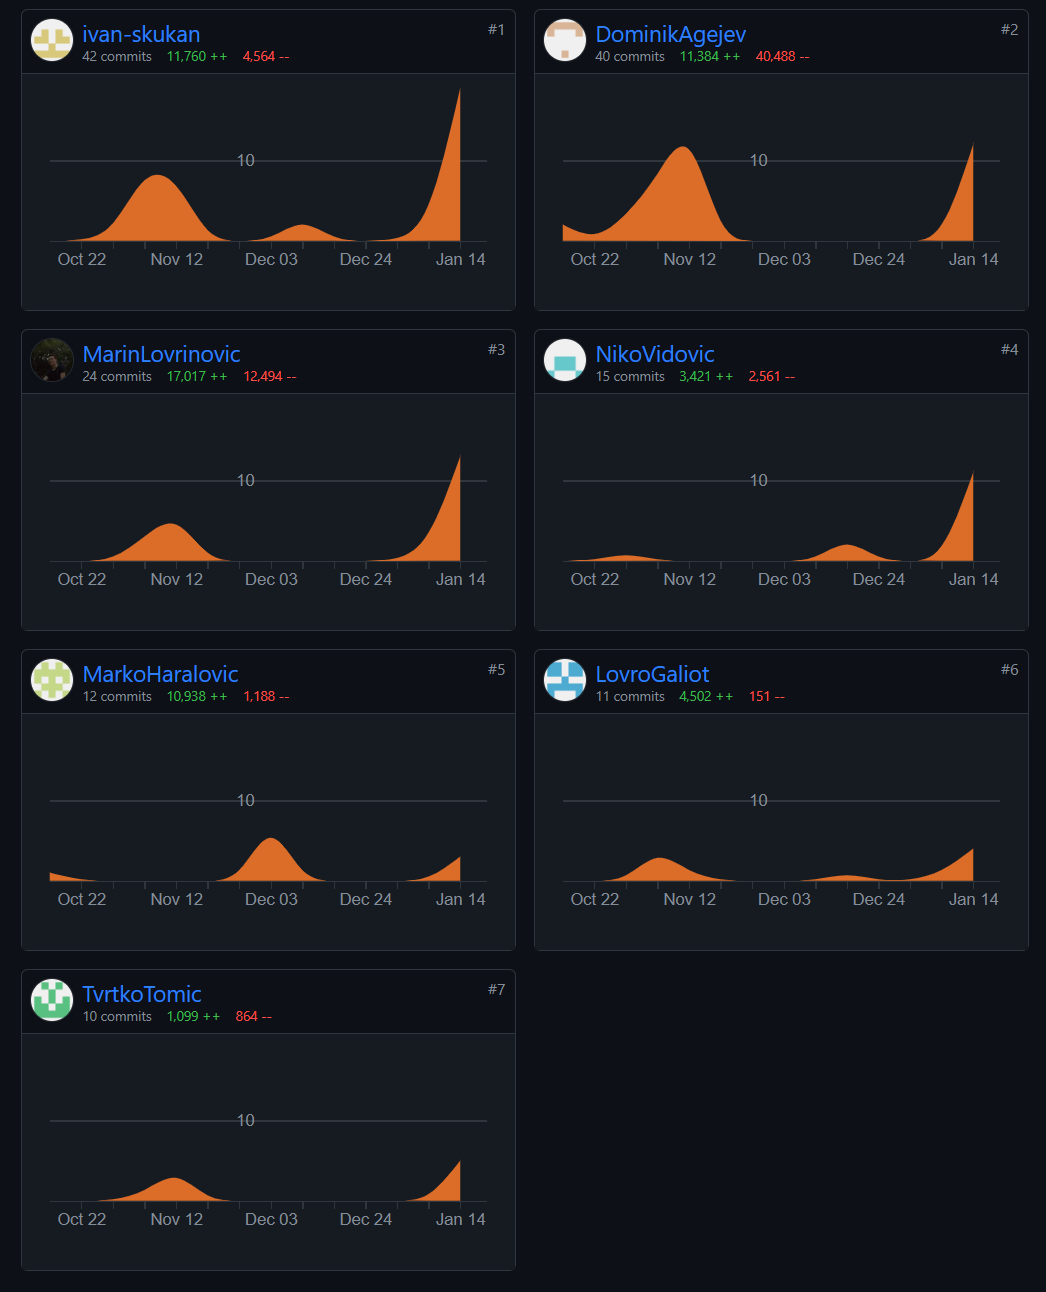
\includegraphics[width=\textwidth]{slike/commits.png}
			\caption{Puštanje aplikacije u pogon preko Visual Studio Codea}
			\label{fig:commits}
		\end{figure}
		
	